\documentclass[11pt]{article}

\usepackage{amsmath, amsthm, amssymb}
\usepackage{graphicx}    % needed for including graphics e.g. EPS, PS
\usepackage{palatino}
\usepackage{tikz}
\usepackage{tikz-qtree}

\usepackage{url, hyperref}


\usetikzlibrary{arrows}
\usetikzlibrary{automata}
\usetikzlibrary{shapes}
\usetikzlibrary{positioning}
\usetikzlibrary{shadows}
%\usetikzlibrary{positioning}


\topmargin -1.5cm        % read Lamport p.163
\oddsidemargin -0.04cm   % read Lamport p.163
\evensidemargin -0.04cm  % same as oddsidemargin but for left-hand pages
\textwidth 16.59cm
\textheight 23.04cm 
%  %\pagestyle{empty}       % Uncomment if don't want page numbers
\parskip 7.2pt           % sets spacing between paragraphs
%  %\renewcommand{\baselinestretch}{1.5} 	% Uncomment for 1.5 spacing between lines
\parindent 0pt		  % sets leading space for paragraphs

% \addtolength{\textwidth}{1in}
% \addtolength{\hoffset}{-1in}
% \addtolength{\textheight}{1in}
% \addtolength{\voffset}{-1in}

\title{\textbf{Tracking and Visualizing Provenance using PostgreSQL}\\
\textsc{6.830 Project : Final Report}}
\author{Alexander Rush (srush@mit.edu)\\ Nirmesh Malviya (nirmesh@mit.edu)}

\begin{document}

\tikzstyle{abstract}=[rectangle, draw=black, anchor=north, text centered]
\maketitle

\begin{abstract}
Many scientific and business applications require keeping detailed track of the origin of data items. Such history is referred to as provenance or lineage of data. The most basic data provenance operations involve tracking which data items an existing data item was derived from (backward data provenance) and what all data items were derived from a given data item (forward data provenance). \\

In this work, we modify the internals of PostgreSQL, a popular open source database, to capture data provenance for a subset of SQL DDL. We have also developed an interactive web interface to query and visualize forward and backward provenance for data items in different databases.
\end{abstract}

\section{Introduction}
% motivate provenance and briefly overview it

A large number of applications such as scientific data management, data integration, information extraction and business analytics involve processing base data to generate a large amount of new data derived from the base data. Capturing which data items contributed to creation of a new data item is important in the face of issues like questionable quality of base data, potential uncertainty associated with it, as well as the authority and trust assessment of the user performing the operations. We see that if data history is not traced in any form as the operations are performed, it would be impossible to track what future tables potential errors in early stage data collection may have propagated to. Tracking down errors and updating all tuples derived from an erroneous data item can be prohibitively costly or even impossible in the absence of this historical information.

% definition of provenance and brief overview
This metadata capturing historical information about a data item is referred to as the \textit{provenance} of the item. The type and amount of provenance information required for different applications vary widely, and depending on the information stored, provenance can be used to derive probabilities associated with a derived data item using uncertainty information about data items that produced it~\cite{widom2005trio}, for debugging schema mappings~\cite{schema_vldb07}, learning authority of data sources~\cite{schema_vldb07}, using user feedback for adjusting ordering in ranking systems ~\cite{integration_vldb08} and many others~\cite{simmhan05asurvey}. Source provenance, a subset of the different types of historical information about a data item, only pertains to what data sources an item was derived from (we can also have transformation provenance, see Section~\ref{background} for a discussion).

% talk about lack of support in databases and current work
Traditionally, attempts to track provenance of data were confined to data processing stages outside of the data management system. With increased availability of cheap storage in recent years and data explosion online (and otherwise), the problem of capturing, storing and querying provenance has been extensively studied~\cite{glavic_dataprovenance, ikeda2010panda, dataspace_halevy}. A number of provenance management solutions have been proposed or developed from the ground up in recent years~\cite{sarma2010live, stonebraker9requirements, widom2005trio, lineage_stanford, chimera_2002, preserv_prov, dbnotes_sig05}. However, to the best of the our knowledge, till date none of the widely used commercial database systems offer even basic support for tracking provenance of all queries executed against the database system. 

In this project, we have added support for tracking source provenance inside a popular open source database system PostgreSQL~\cite{postgres} for a subset of SQL. Our goal is not to compete with existing ground up provenance solutions in terms of efficiency of storing or querying provenance but rather to implement a basic provenance system in a widely used existing large scale system.

In summary, our contributions in this project are:
\begin{itemize}
 \item We implement a basic source provenance system in PostgreSQL, which eagerly captures provenance of newly created data items, allowing for the ability to track provenance using Postgres.
\item We develop an interactive web interface to query forward and backward data provenance on existing tables.
\end{itemize}

The rest of this paper is organized as follows. We explain provenance in Section~\ref{background} and briefly discuss the state of the art in this area in Section~\ref{related}. We describe our implementation in Section~\ref{implement} and show our query interface in Section~\ref{visualizer}. We finally conclude in Section~\ref{conclude}.


\section{Background} \label{background}
% add background on what provenance is 
% add a diagram

% \begin{figure}
%   \centering
%   \label{diag}
%   \begin{tikzpicture}
%     \node (s1) [draw]{s1};
% 
%     \node (s2) [draw,above right= of s1]{s2};
%     \node (s3) [draw,below right= of s1]{s3};
%     \node (s4) [draw, right= of s3]{s4};
%     \path [->] (s1) edge[thick] (s2);    
%     \path [->] (s1) edge[thick] (s3);    
%     \path [->] (s3) edge[thick] (s4);    
% 
%     \path [->] (s4) edge[thick, bend right = 50, dotted] (s3);    
%     \path [->] (s3) edge[thick, bend right = 50, dotted] (s1);    
%   \end{tikzpicture}
%   \begin{tikzpicture}
%     \node (s1) [draw]{s1};
% 
%     \node (s2) [draw,above right= of s1]{s2};
%     \node (s3) [draw,below right= of s1]{s3};
%     \node (s4) [draw, right= of s3]{s4};
%     \path [->] (s1) edge[thick] (s2);    
%     \path [->] (s1) edge[thick] (s3);    
%     \path [->] (s3) edge[thick] (s4);    
% 
%     \path [<-] (s4) edge[thick, bend right = 50, dotted] (s3);    
%     \path [<-] (s3) edge[thick, bend right = 50, dotted] (s1);    
%     \path [<-] (s2) edge[thick, bend right = 50, dotted] (s1);    
%   \end{tikzpicture}
% 
%   \caption{(a) Backward provenance (b) Forward provenance}
% 
% \end{figure}

The term \textit{provenance} or \textit{lineage} of data broadly refers to what source a data item came from, what transformations were applied on the original data to arrive at the current data item, how the current data item has been updated over time and what other data items might have been derived from the current data item. Broadly speaking, provenance information belongs to one of two categories: \textit{source provenance} and \textit{transformation provenance}~\cite{tan_ieee04}. Source provenance refers to source data from which a data element was derived, whereas transformation provenance is concerned with the different processes or operations that were used to arrive at the data element starting from the source data. A slightly different characterization~\cite{ikeda2010panda} classifies provenance as mostly either \text{data-based}, in which well defined data models are used to track fine-grained provenance of data elements, or \text{process-based}, where the processes generating a data element along with coarse-grained provenance is captured. 

The proposal for the SciDB project\cite{stonebraker9requirements} lists three requirements for a useful provenance system:

\begin{itemize}
\item For any data element, we would like to recover the \textbf{derivation history}. This would be helpful in identifying if a data element originated from a suspect or unreliable data source.
\item If a data element is found to have had value some value in error, we would like to trace forward to see what other data elements could have been affected from the element's previous erroneous value. If a portion of data is identified as erroneous, we can use this to determine what other data elements in the data store have values that cannot be relied on as a result of this.
\item At any point, we would like to reproduce the construction of the current data in the data store. This would be of use in propagating updates downstream when data element errors are identified and corrected.
\end{itemize}

Thus we can have two types of provenance queries, \textit{forward} and \textit{backward} provenance. In forward provenance, given some data element, we ask what data elements were produced from it (and optionally what processing operations were applied to them during the element's creation). In backward provenance, given some data element, we ask where it originally came from (and optionally what processing led to its creation). 

Fig~\ref{diag} shows examples of these two queries. We assume that our original data is $s1$, it leads to $s2$ and $s3$. In turn, $s4$ is derived from $ s3$. Our forward query from $ s1$ leads to each of the other data elements, while the backward query from  $s4$ leads back to the root. 

Provenance can either be computed and stored eagerly by capturing forward and backward data pointers (for example~\cite{widom2005trio}) or lazily by just recording the query log along with a knowledge of inversion operations~\cite{stonebraker9requirements}. 

A more detailed survey of data provenance approaches, including a discussion of conceptual properties of provenance models and different storage and recording strategies can be found in \cite{glavic_dataprovenance}. The two strategies have vastly different storage requirements and query efficiency. We discuss some work on this in Section~\ref{related}.

 \section{Related Work}	\label{related}
% detail each work briefly. There is nothing to dismiss really.


In particular, we hope to respond to the challenge given by \cite{cudré2009demonstration}.

\begin{quote}
Recording the log is easy. The hard part is to create a provenance query language and an efficient implementation.  
\end{quote}

Recent work in this area includes the Trio/LIVE system and the Panda project. However, neither of these projects handle backward provenance efficiently or provide language support for querying provenance.
This lack of historical record can make database systems impractical for scientific research. 

One practical issue with available database systems is the difficulty of tracing data history. 

~\cite{buneman00}

\cite{simmhan05asurvey} 

\cite{simmhan_survey} 

\cite{glavic_dataprovenance}

\cite{queryprov_sig2010}

\cite{chapman_provstorage, buneman00, simmhan05asurvey}

\cite{plt_stanford}

\begin{itemize}
%\item Trio / LIVE \cite{} 
  
\item Implements a technique for backward provenance by connecting derived tuples to the previous tuples. Unfortunately, this technique has very high space complexity and may not scale in practice. 

\item Panda \cite{ikeda2010panda} 

Panda is an early stage proposal for a general provenance system for data. This system does not propose a practical algorithm or language features for provenance. 

\item SciDB \cite{cudré2009demonstration}

The SciDB system proposes a provenance system. Current proposals have low space complexity but with non-trivial query time. 

\end{itemize}


In the LIVE provenance system built as part of the Trio project, the database stores a back pointer for each derived data element. In our example, it would store $(s1, s2)$, $(s1, s3)$, and $(s3, s4)$ explicitly. It can then perform very efficient backwards queries by walking along this tree. Unfortunately, this technique requires storing a derivation pair for each derived and its parents, which can be very expensive.  

The SciDB proposal suggests a different way to implement provenance. For forward queries, the propose using the databases version control system and following forward deltas. They note that backward provenance is more difficult to implement. Two possible methods they mention are to also include backward deltas as part of version control or to implement an algorithm which can reverse the queries from the log. 

The other open quesion surrounding provenance is how to include provenance queries within SQL. There have been relatively few proposed solutions for this problem. The LIVE system implements a keyword ``valid at'' which queries a data element at a specific revision. For instance the query:

\begin{verbatim}
SELECT * FROM <table-name> VALID AT <revision-number>
\end{verbatim}

This query returns the rows from a table at a specific revision number. This syntax allows a query to access a revision, but does not allow us to specify a provenance query the directly. 


\section{System Architecture} \label{archi}

\begin{figure}
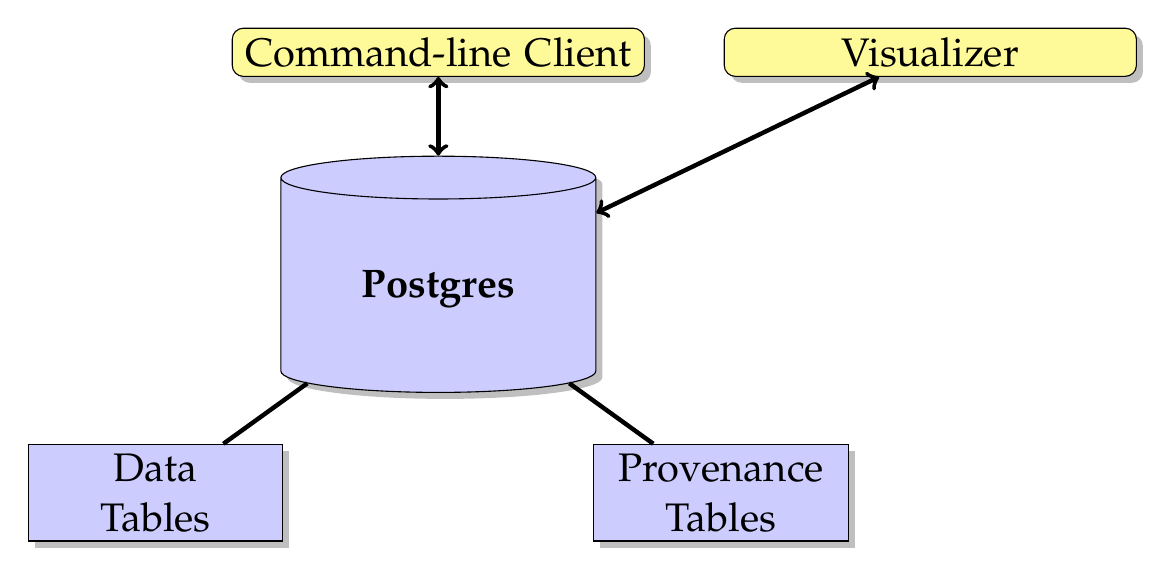
\begin{tikzpicture}[node distance=1cm, font=\Large]
  \tikzstyle{box}=[drop shadow, rectangle, fill=yellow!40, rounded corners, draw=black, anchor=north, text centered, text width=5cm]
  \tikzstyle{pbox}=[drop shadow, fill=blue!20, draw=black, anchor=north, text centered, minimum height=3.0cm, minimum width=4.0cm]
  \tikzstyle{sbox}=[drop shadow, rectangle, fill=blue!20, draw=black, anchor=north, text centered, text width=3cm]
  \node (post) [pbox,cylinder, shape border rotate=90, aspect=0.25, ]{\textbf{Postgres}};   
  \node (data) [sbox, rectangle, below left=of post, text centered ]{Data\\  Tables};   
  \node (prov) [sbox, below right=of post, text centered]{Provenance\\ Tables };   


  \node (client) [box, above=of post ]{Command-line Client};           
  \node (vis) [box, right=of client]{Visualizer};           

  \draw[<->, ultra thick] (vis) --(post);
  \draw[<->, ultra thick] (client) --(post);
  \draw[-, ultra thick] (prov) --(post);
  \draw[-, ultra thick] (data) --(post);
\end{tikzpicture}

\caption{The architecture of our provenance system}
\label{fig:provarch}
\end{figure}

Figure~\ref{fig:provarch} shows the architecture of our provenance system. Provenance tables are populated as the PostgreSQL backend executes queries which add new tuples to the database. Each database has its own dedicated provenance store which tracks provenance for all tables inside the database. The eagerly captured provenance information can be queried via both command line and graphical interfaces. Querying forward and backward provenance via command line requires jointly querying against the provenance and data tables using the table name and id of the data tuple under consideration. 

The graphical interface is a web-frontend which queries the provenance tables for forward and backward provenance in the background as the user interactively clicks on data elements of interest. Different tables and data elements can be directly specified using their names/ids using drop-down HTML forms (see Section~\ref{visualizer} for details). 


\section{Tracking Provenance inside PostgreSQL} \label{implement}

% may be add code snippets here to give a preview of some stuff that had to be done inside Postgres
Catalog

\subsection{Simple selects - queries on One Table}

\subsection{Handling joins}

\subsection{Aggregates}

\subsection{Changes to the storage manager for disk based workloads}


\section{Visualizing Forward and Backward Provenance} \label{visualizer}

\input{visual}

don't support stored procedures , they are black boxes, and unless something useful is known about the underlying functions, we anyway do not get to know too much about them.

%\section{Experiments}

%three graphs -- CPU, memory and storage overhead of tracking provenance averaged over a certain number of queries over the usual

\section{Conclusion and Future Work}	\label{conclude}

In this project, we extended PostgreSQL by adding native support for a provenance system which required modified postgres internals. The system we have implemented eagerly captures evolution history of tuples as various queries are run against the system. To this end, we modified the query execution engine of PostgreSQL to track provenance information up along various nodes in the query execution plan tree. We also changed the internal storage engine to store provenance information as it writes bare-minimum tuples to disk for various disk based operations (disk-based sort for example).

Through our work, we have handled a subset of SQL DDL, and support SELECTS, PROJECTS, JOINS, AGGREGATES (including GROUP BY and ORDER BY).  We however do not support stored procedures, for they are black box functions external to the database and the input data elements into the function are all that is known to the executor at run time, allowing us to capture only coarse-grained provenance information for the output data elements. 

As future work, we hope to be able to address this limitation. Measuring and profiling the CPU and storage overhead of tracking provenance in Postgres and the performance impact on the system for standard workloads would also be an interesting direction to pursue.



\bibliographystyle{acm}
\bibliography{prov}
\end{document}